\documentclass[11pt,conference,compsocconf]{IEEEtran}

\usepackage{hyperref}
\usepackage{graphicx}	% For figure environment
\usepackage[english]{babel}
\usepackage{tabu}
\usepackage{xargs}  
\usepackage{float}
\usepackage{listings}
\usepackage[prependcaption,textsize=tiny]{todonotes}
\presetkeys{todonotes}{inline,backgroundcolor=red}{}


\begin{document}
\title{Class Project 2 Report: Road Segmentation Challenge}

\author{
  Angerand Gr\'egoire, Goullet Boris, Grondier Julien 
}

\maketitle

\begin{abstract}
In this project, we were given a dataset consisting of aerial photographs of suburban areas. Our task was to apply different machine learning methods to this dataset to train a model that would predict where roads were present in these photographs.

Using a Convolutional Neural Network and image processing algorithms, we achieved 82.9 F\textsubscript{1}-score.
\end{abstract}


\section{Models applied}

\subsection{Logistic regression}
At first, we tried using a logistic regression. We did this by cutting up the images into small patches (either 4x4, 8x8, or 16x16) and training a logist model on 3 features for that patch: mean Red pixels values, mean Green pixel values, and mean Blue pixel values.

However, results were less than satisfactory, even with more/different features or patch sizes, so we quickly dropped that idea.

\subsection{Convolutional Neural Network}
We thus turned our focus to CNNs. We started off by using the provided code from \texttt{tf\_aerial\_images.py}.

We played around with its parameters and noticed that we had much better results with a patch size of 4x4, instead of the default 16x16. We also reduced the size of its convolution filters to 4x4 instead of 5x5, to match the patch size.

\subsubsection*{Custom CNN classifier}
We then tried building our own Convolution Neural Network rather than using the provided one, for better modularity. We were aiming for the architecture in Figure \ref{fig:custom_CNN}.

\begin{figure}[h]
\centering
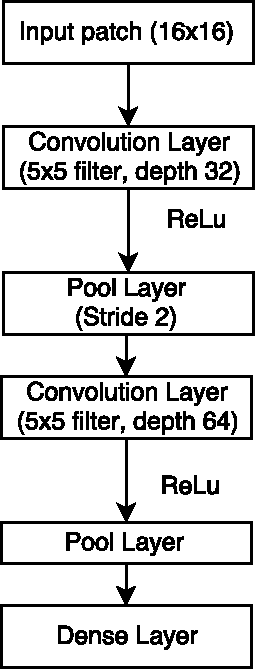
\includegraphics[height=0.5\textheight,keepaspectratio]{custom_CNN.pdf}
\caption{Architecture of our attempted custom CNN}
\label{fig:custom_CNN}
\end{figure}

However, after a lot of debugging, we failed to achieve anything and had to fallback on the provided file. The code can be checked in \texttt{custom\_classifier.py}

\section{Feature pre-processing}

Our CNN works on sub-patches of 4x4x3 (RGB) of the training images with labels from the corresponding ``groundtruth'' patch.

We train the CNN by cutting up 500 different source images: the 100 given as a dataset, plus variations of those (transposed, flipped horizontally, flipped vertically, and flipped both vertically and horizontally).

Furthermore, we tried adding a new label as groundtruth, manually annotated, corresponding the the position of roofs. However, this did not improve prediction rate compared to having only `background' and `road' as labels.


\section{Results post-processing}
After obtaining the raw prediction from the convolutional neural network, we do a post-processing step in order to remove most of the noise.

The post processing consists of a convolution, using a cross shaped kernel. This shape has be chosen to match the many right angle intersections present in our dataset.


In some cases the roads are not aligned to the image axes, to handle those we extract the most significant straight lines from the image using Hough transform and rotate our kernel to match their orientation.

\begin{figure}[h]
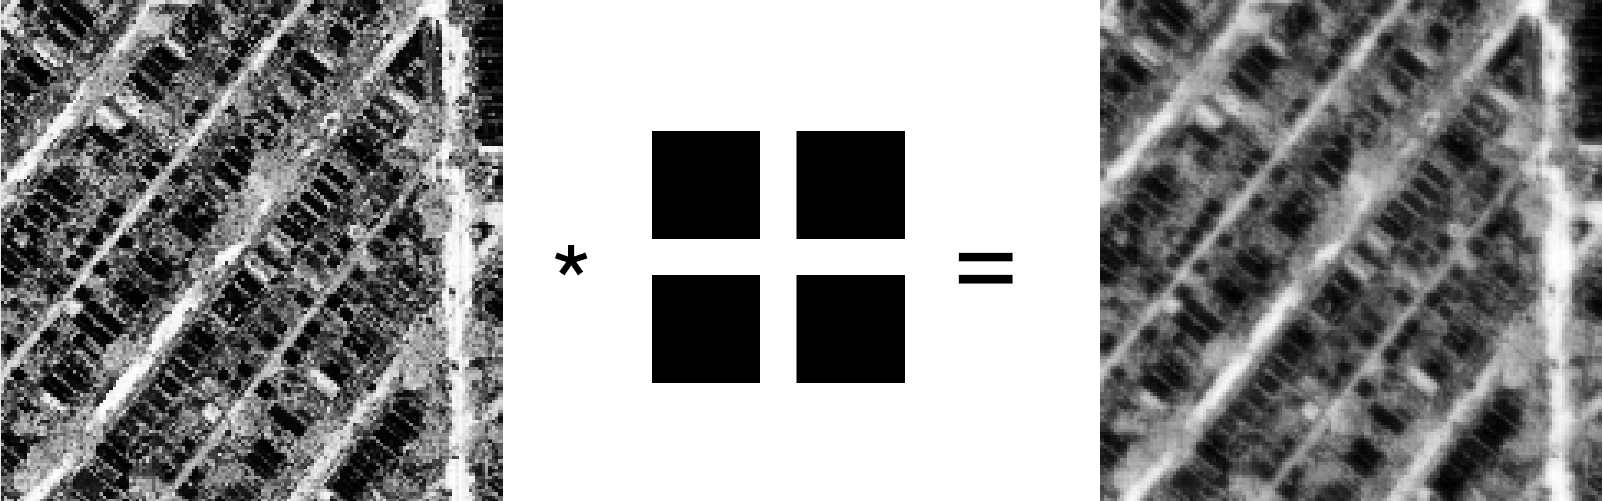
\includegraphics[width=0.5\textwidth]{conv.png}
\caption{Prediction convolution}
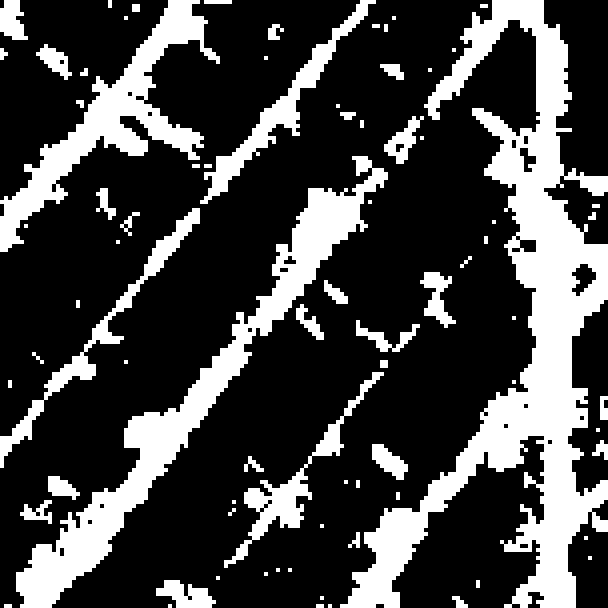
\includegraphics[width=0.5\textwidth]{50_final_mask.png}
\caption{After thresholding}
\end{figure}

\section{Discussion}
We remark that our model has a hard time differentiating flat, grey roofs from the road, probably because those are expansive grey surfaces, exactly like roads. Car parks are also often marked as roads, as they are, in effect, private roads --- in our opinion, car parks should be considered roads, despite what the training set states.

Our model also misses roads when they are covered by a large tree --- although technically one can't be sure there is a road under it, we just infer its probable presence from the presence of two road parts on either side. Furthermore, when a road is very thin and very close to the buildings surrounding it (e.g. European cities' historical centers) it is often not detected.

\section{Summary}
While we had high hopes for using a custom CNN architecture, we are disappointed that we weren't able to build a functional one. However, using the basic, provided CNN, we achieved results that we would deem satisfactory.

\end{document}
